%\usepackage{subfig}

\chapter{Observations and Analysis}

In order to study this problem about the dynamics of Globular Clusters in our galaxy we need scientific data that allows us to build a model that fits our observations. Under supervision of professor Juan Carlos Mu\~noz Cuartas and with three other undergraduate students from the University of Antioquia a trip to the OPD (Pico dos Dias Observatory) was made to Brazil in May 2014, besides the observational experience of the students, the main purpose of the trip was to get important data for this project. We needed two sets of data corresponding to spectra and photometric images of different Globular Clusters

The spectroscopic data allows us to determine the relative motion of individual stars (in the case of individual spectra) to infer the velocity dispersion profile. The integrated spectra can give us information about the stellar populations and it can also be used to infer composite velocity dispersions due to the Doppler broadening of the spectral lines. The photometric data allows us to study the surface brightness distribution for them. We can use all of this information to infer the properties of the globular clusters' mass distribution in order to build complete dynamical models and therefore infer the amount of dark matter present in the globular clusters (if there is any).

\section{Observational Procedures}

Our stay in OPD consisted of two days in the main dome for the spectroscopic data (using the Perkin-Elmer (P\&E) telescope with a 1.6m mirror and the Cassegrain Spectrograph) and four days in a smaller dome for the photometric data in the IAG telescope with a 0.6m mirror. Figure 3.1 shows the configuration of telescopes in the observatory.

\begin{figure}[H]
\centering
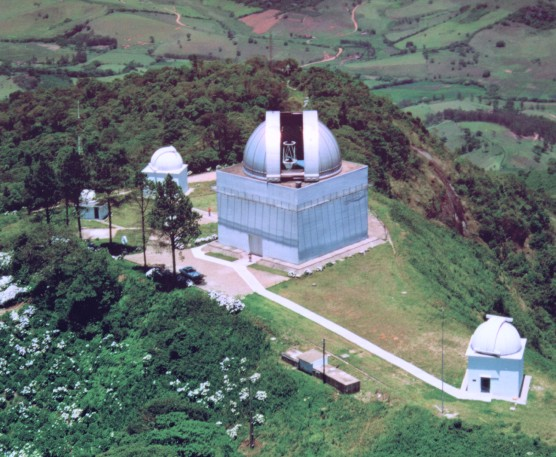
\includegraphics[width=10cm]{images/opd.jpg}
\caption[OPD Observatory]{OPD observatory seen from the air, the big dome was used for the spectroscopic data and the small dome at the low right part of the photo for the photometric data.}
\end{figure}

\subsection{Spectroscopic Data}

The first two days (May 14th and 15th) we took the spectroscopic data in the telescope P\&E with a diameter of 1.6m. The main instrument was the Cassegrain spectrograph with a CCD Ikon-L camera and Filters UBVRI. The control software we used was the recently installed software TCSPD which is built in a LabView environment for Windows (2010). Figure 3.2 shows the telescope from inside the dome.

\begin{figure}[H]
\centering
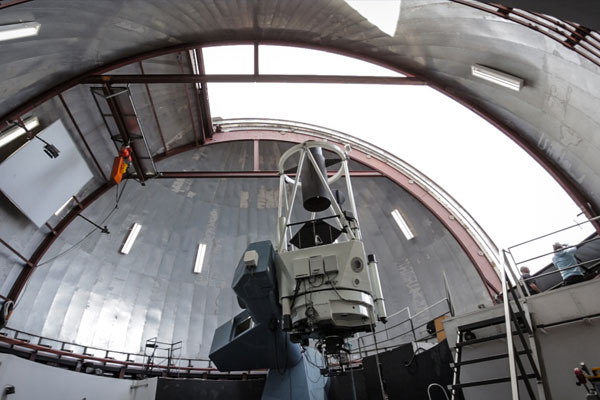
\includegraphics[width=10cm]{images/opd-spectrograph.jpg}
\caption[Perkin-Elmer telescope used for Spectroscopy]{Perkin-Elmer telescope in the main dome in OPD used for the spectroscopic observations}
\end{figure}

We made the observations of dome flats, bias frames, comparison lamp frames, calibration stars, some galaxies and certain globular clusters of the milky Way organized by the best observation times using Simbad and Stellarium for the estimations of the coordinates and times respectively. The objects we observed in OPD are organized in Table 3.1.

\begin{table}[H]
\begin{center}
  \begin{tabular}{| c| c| c| c| c| c| c| c| }
    \hline
    \textbf{Object} & $\boldsymbol\alpha$ & $\boldsymbol\delta$ & \textbf{14$^{th}$} & \textbf{15$^{th}$} & \textbf{16$^{th}$} & \textbf{18$^{th}$} & \textbf{19$^{th}$} \\ \hline
    NGC5020 & 13h 12m 39.87s & +12$^{\circ}$35'59.0" & \checkmark & \xmark & \xmark & \xmark & \xmark \\ \hline
    NGC5272 & 13h 42m 11.62s & +28$^{\circ}$22'38.2" & \checkmark & \checkmark & \checkmark & \xmark & \xmark \\ \hline
    NGC4833 & 12h 59m 33.92s & -70$^{\circ}$52'35.4" & \checkmark & \xmark & \xmark & \xmark &\xmark \\ \hline
    NGC4590 & 12h 39m 27.98s & -26$^{\circ}$44'38.6" & \checkmark & \checkmark & \checkmark & \xmark & \checkmark\\ \hline
    NGC5139 & 13h 26m 47.28s & -47$^{\circ}$28'46.1" & \checkmark & \checkmark & \checkmark & \checkmark & \checkmark\\ \hline
    NGC5286 & 13h 46m 26.81s & -51$^{\circ}$22'27.3" & \checkmark & \checkmark & \xmark & \xmark & \checkmark\\ \hline
    NGC6752 & 19h 10m 52.11s & -59$^{\circ}$59'04.4" & \checkmark & \xmark & \xmark & \xmark & \xmark \\ \hline
    NGC6397 & 17h 40m 42.09s & -53$^{\circ}$40'27.6" & \checkmark & \checkmark & \checkmark & \xmark & \checkmark\\ \hline
    NGC6723 & 18h 59m 33.15s & -36$^{\circ}$37'56.1" & \checkmark & \checkmark & \xmark & \checkmark & \checkmark\\ \hline
    NGC7615 & 23h 19m 54.44s & +08$^{\circ}$23'57.9" & \checkmark & \xmark & \xmark & \xmark & \checkmark\\ \hline
    NGC6541 & 18h 08m 02.36s & -43$^{\circ}$42'53.6" & \checkmark & \checkmark & \xmark & \checkmark & \checkmark\\ \hline
    NGC2802 & 09h 16m 41.41s & +18$^{\circ}$57'48.8" & \xmark & \checkmark & \xmark & \xmark & \xmark \\ \hline
    NGC5024 & 13h 12m 55.25s & +18$^{\circ}$10'05.4" & \xmark & \checkmark & \xmark & \xmark & \xmark \\ \hline
    NGC6362 & 17h 31m 54.99s & -67$^{\circ}$02'54.0" & \xmark & \checkmark & \xmark & \xmark & \xmark \\ \hline
    NGC6502 & 18h 04m 13.68s & -65$^{\circ}$24'35.7" & \xmark & \checkmark & \xmark & \xmark & \xmark \\ \hline
    NGC7078 & 21h 29m 58.33s & +12$^{\circ}$10'01.2" & \xmark & \checkmark & \xmark & \checkmark & \xmark \\ \hline
    NGC7099 & 21h 40m 22.12s & -23$^{\circ}$10'47.5" & \xmark & \checkmark & \xmark & \xmark & \xmark \\ \hline
    NGC6970 & 20h 52m 09.46s & -48$^{\circ}$46'39.8" & \xmark & \xmark & \xmark & \xmark & \checkmark\\ \hline
    NGC6541 & 18h 08m 02.36s & -43$^{\circ}$42'53.6" & \xmark & \xmark & \xmark & \xmark & \checkmark\\ \hline
    NGC6715 & 18h 55m 03.33s & -30$^{\circ}$28'47.5" & \xmark & \xmark & \xmark & \xmark & \checkmark\\ \hline
    HR4963 & 13h 09m 56.99s & -05$^{\circ}$32'20.4" & \checkmark & \xmark & \xmark & \xmark & \xmark \\ \hline
    HR4468 & 11h 36m 40.91s & -09$^{\circ}$48'08.1" & \checkmark & \checkmark & \xmark & \xmark & \xmark \\ \hline
    HR7950 & 20h 47m 40.55s & -09$^{\circ}$29'44.8" & \xmark & \checkmark & \xmark & \xmark & \xmark \\ \hline
    HR4961 & 13h 09m 45.28s & -10$^{\circ}$19'45.6" & \xmark & \xmark & \checkmark & \xmark &\xmark \\ \hline
    HR6308 & 16h 59m 57.71s & -25$^{\circ}$05'31.9" & \xmark & \xmark & \xmark & \checkmark & \checkmark\\ \hline
    HR7964 & 20h 49m 20.54s & -18$^{\circ}$02'09.1" & \xmark & \xmark & \xmark & \checkmark & \xmark \\ \hline
    HR6386 & 17h 12m 13.62s & -25$^{\circ}$15'18.6" & \xmark & \xmark & \xmark & \xmark & \checkmark\\
    \hline
  \end{tabular}
\end{center} 
\caption[Observed objects in OPD]{Observed objects in OPD observatory, the table contains the equatorial coordinates of the objects and the days each object was observed, the check mark indicates that the object was observed and the x mark indicates it was not observed. The details of the observations for each day are explained right ahead.}
\end{table}

Now, our set up configuration for the spectrograph was the following:

On May 14th, a diffraction grating of 900 lines per mm, a CCD IkonL and the central wavelength for the observations of 8500 Angstroms (with possibility of rotation of the slit 90°, +45° and -45°). We used the slit of 2.52" and obtained data for the globular clusters: NGC5020, NGC5272, NGC4833, NGC4590, NGC5139, NGC5286, NGC6752, NGC6397, NGC6723, NGC6715 and NGC6541 using exposition times of 600 and 900 seconds. We also observed the calibration stars: HR4963 and HR4468 with exposures of 7 and 5 seconds. As it was the first day, we needed to be very careful in calibrating our instruments on order to have the objects in the right focus, we also made the rotation of the slit to use all the diffraction angles of the observations and our comparison lamps were of Ne-Ar.

On May 15th, we used the slit of 3.0", and used a central wavelength of 5500 Angstroms. This time we observed the following objects: NGC2802, NGC5024, NGC4590, NGC5139, NGC5286, NGC5272, NGC6362, NGC6397, NGC6723, NGC6502, NGC6541, NGC7078, NGC7099, the stars HR4468 and HR7950. We used pretty much the same exposition times than the day before, this time though, our comparison lamps were or He-Ar.

\subsection{Photometric Data}

The photometric data was acquired in the next four days (from May 16th to May 19th) in the 0.6m IAG telescope in OPD. We used the Johnson system for the different filters which were easily shifted with the given software in the control computers. Figure 3.3 shows the telescope from inside the dome.

\begin{figure}[H]
\centering
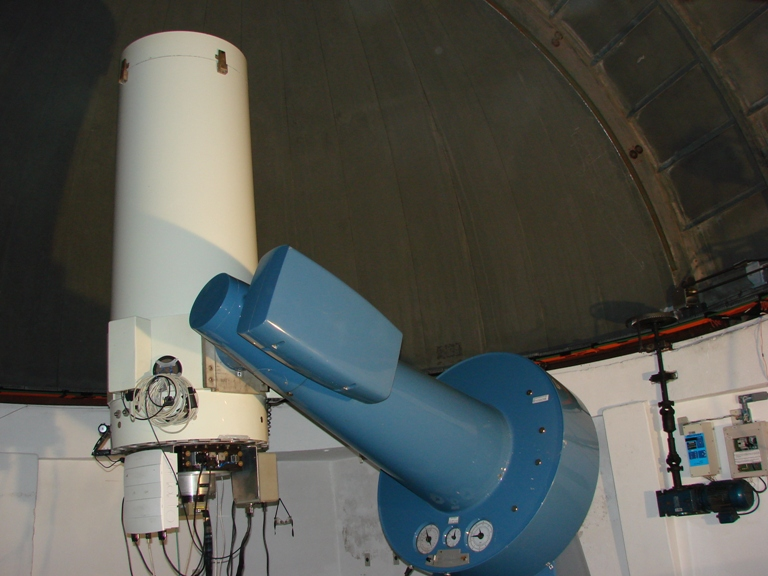
\includegraphics[width=8cm]{images/opd-photometry.jpg}
\caption[IAG Telescope used for Photometry]{IAG telescope used for the photometric data}
\end{figure}

On May 16th, we took all the calibration images, consisting of 20 bias frames with an exposition time of 0,00001 seconds; also 22, 11, 11, 20 and 10 flat frames for the B,I,R,U,V filters respectively, their exposition times differed, for  U filter we took various frames of 60 and 30 seconds, for the B filter we took frames of 30 seconds each, 15s for I, 60s for R and 3s for V. We took our ``focus" images to calibrate the instrument, and also various skyflats for all the filters. We targeted the following globular clusters and calibration stars in different filters: NGC5272, HR4961, NGC4590, NGC5139 AND NGC6397. The exposition time for the clusters was of 600 seconds and 2 and 4 seconds for the calibration star. 

May 17th was a terrible night for observations because the sky was too cloudy and the only useful data we could get were dome flats for the filters I,R and V that we could use instead of the bad dome flats of the first day. The reduction using the flats of another day are decent but this is not the ideal situation since mechanical movements of the instrument might slightly change its configuration and therefore it probably ends up with a reduction that is not the ideal one for science purposes.  

On May 18th we were more organized since we were getting familiar with the observations and therefore the data we got had little trouble in the upcoming analysis, even though the sky was clody at the end of the night. The science objects we observed were NGC5139, HR6308, NGC6723, NGC6541, NGC7078, HR7964 that were observed in the different filters. We got 20 bias frames, 14 dome flats in the vaious filters, but no skyflats. 

On May 19th we observed the Clusters NGC5139, NGC4590, NGC6723, NGC6715, NGC6541, NGC6970, NGC5286,    NGC6397, NGC6541 and NGC6715, the calibration stars HR6386 and HR6308, 20 bias frames and flats for each filter.

\section{First step for Anaysis}

Our first goal in starting the analysis of all the relevant data was to organize all the images in order to reduce the time required to make the reductions. For every day the calibrations images, trash, calibration stars and objects were separated and they were given their correct names as they were in the headers and compared with the information sheets we filled at the time we were doing the observations.

The next step was the reduction of all the images with the calibration files for each day, I started the photometric data to acquire certain skills in the use of IRAF because the reduction of the spectroscopic data was a little more complex and needed a deeper understanding of IRAF packages. 

We started with the cluster NGC-5139 ($ \omega $ Centauri) because we got lots of data for that cluster in OPD and also because $ \omega $ Centauri is a well known globular cluster since it is the largest in our galaxy and we can get a lot of information from the databases. 

After the photometry of that cluster, the most relevant part of the reduction was to be made. The reduction and analysis of the spectroscopic data (May 14th and 15th), the methods for these reductions are quite special and are the most relevant part of the analysis because that is our most valuable information. The reduction was to be made very carefully because a good spectroscopic analysis depends upon a good reduction of the data. Just as with the photometric data, the first procedures were made for the Cluster NGC5139 to understand and master the techniques of the reduction and extractions.

\section{Photometry}

The photometry was made by the two traditional methods, PSF photometry and Aperture Photometry; even though the magnitudes calculated using both methods are quite different, the calibration constant between the two methods gave a good relation between them and made us trust the photometry results.

But first, the reduction of the data had to be done. The first step is to characterize the calibration images in order to see if there are any errors associated with the instrument or the way that the observations were made. By doing this we found that most of the flat-field images had brightness gradients in the corners and this was a problem we needed to correct because the increased value on the counts in these corners would affect the normalization of the super-flat that we would use to reduce the science data. Another systematic error that we found in all of our calibration and science frames was the presence of a strange water-looking figure at the top left corner of them, although it can be removed with the correct reduction, it obviously affected the CCD sensitivity by the time of the observations. Also, some filters showed a higher sensitivity to this systematic errors but at the end, the photometry could be made in the best data so that the dirty images don't affect our results.

In order to see how the data would be affected by the systematic errors we just mentioned, we produced a composite image using three images with the filters U,V and R and we did the same with the flats in those filters, the results are shown in figures 3.4 and 3.5.
  
\begin{figure}[H]
  \centering
  \begin{minipage}[b]{0.47\textwidth}
    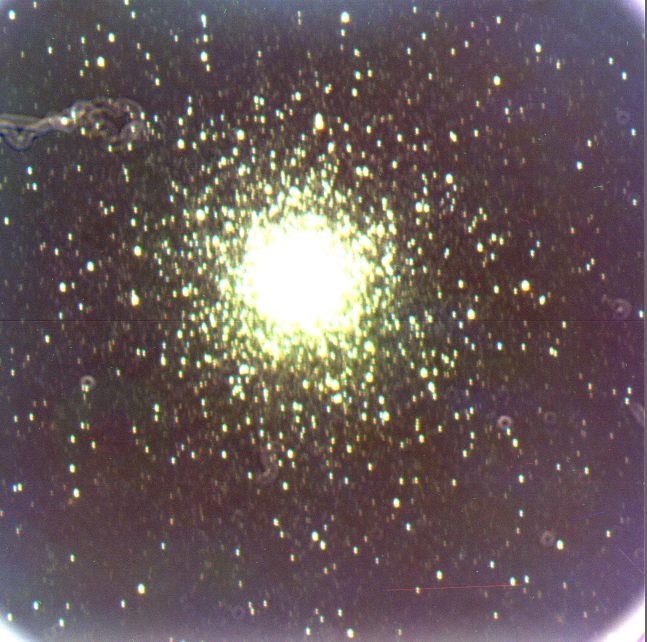
\includegraphics[width=\textwidth]{images/ngc_5139_dirty.png}
    \caption[Dirty image of NGC5139]{Composite image of NGC5139 without being previously reduced}
  \end{minipage}
  \hfill
  \begin{minipage}[b]{0.47\textwidth}
    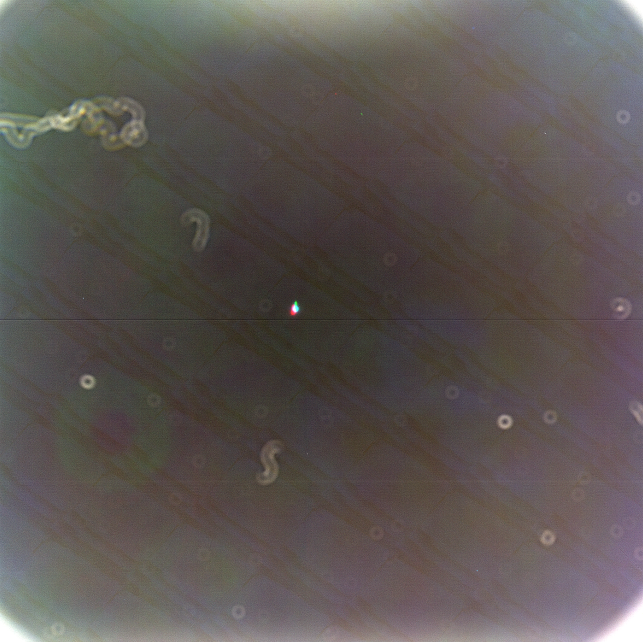
\includegraphics[width=\textwidth]{images/ruido.png}
    \caption[Clean image of NGC5139]{Composite image of the flats showing the noise that needs to be extracted}
  \end{minipage}
\end{figure}

What we can infer from these images is that the flat fields and the bias frames contain the same noise that the science data thus giving us a good result in the reduction.

Once all the characterization is made we can reduce our important data using IRAF following the conventional steps consisting of: 

- Building a Superbias: \textit{Zerocombine} allows us to create the superbias using the median.

- Substracting the Superbias to every flat and science data: We substract the Superbias to every flat frame with no distinction on the filter, this is easily made using the task \textit{imarith}, we also substract them from the original science images.

- Building Superflats: It is necessary to create a Superflat frame for each filter because the response of the CCD and will be different for different wavelengths, we use the task \textit{imcombine} to do this and this time we use the mode for better results.   

- Divide the Superflats by the median: In order to normalize the flatfields we find the mode of each frame with \textit{imstatistics} and then divide them by that value


\begin{figure}[H]
\centering
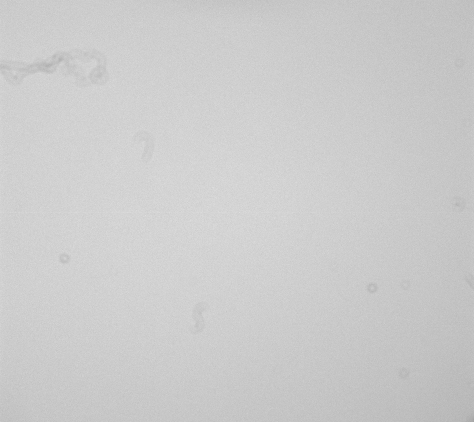
\includegraphics[width=8cm]{images/flat_I.png}
\caption[Normalized Superflat for the filter I]{Example of one of the Normalized Superflats for the I filter}
\end{figure}

- Reduce the science data: Finally, we divide the original images of the clusters and stars (with the bias substractet) by the normalized Superflat to get the reduced images. This can easily be made using the task \textit{imarith}.

\subsection{Aperture Photometry}

Now that the reduction has been made and the corrections pixel by pixel have been applied, we can proceed to do the photometry using the simplest technique, known as Aperture Photometry which consists of adding up the pixel counts within a circle centered on each star of the cluster and subtracting the quotient of the per-pixel average value of nearby sky count divided by the number of pixels within the aperture. This will result in the raw flux value of the target object. This Aperture Photometry was done using the task \textit{Phot}:

For stars in $\omega$ Centauri, one must choose a very small aperture of the sky because the surrounding stars contribute to the flux that needs to be extracted and they are very close to each other, the crowded region of the center of $\omega$ Centauri is shown in figure 3.7. 

\begin{figure}[H]
\centering
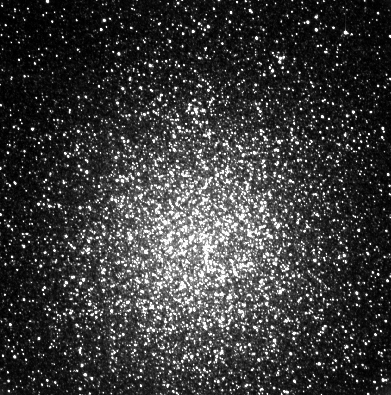
\includegraphics[width=8cm]{images/NGC5139_red.png}
\caption[NGC5139 as observed in the V filter]{One of our observations of NGC5139 in the V filter with an exposition time of 480 seconds}
\end{figure}

With the task \textit{imexamine} I find a value for the FWHM of 6.4 which I will use to set the size of the apertures to do the photometry. For the size of the aperture containing each star I chose an aperture size of four times the FWHM of the point spread function associated to the stars because it is the one that best fits the photometry and minimizes the error (calculated for some stars pressing ``a" with the \textit{imexamine} task) and for the width of the aperture I chose I value of 2.5 times the FWHM.

Another important value to take into account before editing the parameters in \textit{phot} is the medium value of the background on the sky, in the case of this cluster, I do an average on many different places in the background of the image and find a value of sigma for the image that is equal to 53.45.

Now the photometry is done by changing some of the parameters including the readnoise and the gain. In the \textit{fitskyparts} task inside phot I set the inner radius called annulus to be 25.6 (4FWHM) and the intermediate width called dannulus of 16 (2.5FWHM). Finally, before running the task I make sure I do the photometry using various apertures because I want to see which one minimizes the errors. I set apertures to be 1FWHM, 1.5FWHM, 2FWHM, 2.5FWHM, 3FWHM, 3.5FWHM and finally run the task. The results of the magnitude found for one of the star as a function of the size of the aperture is displayed in figure 3.8.

\begin{figure}[H]
\centering
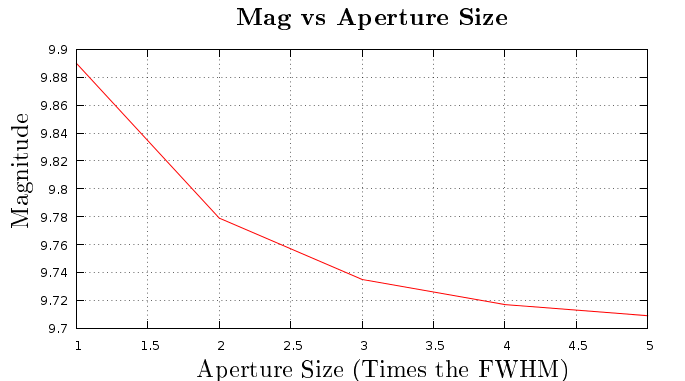
\includegraphics[width=12cm]{images/mag_vs_ap_size.png}
\caption[Photometry results of Magnitudes vs Size of apertures]{The magnitude decreases for bigger appertures}
\end{figure}

As we can see in figure 3.8, the magnitude of the chosen star in the cluster decreases for bigger apertures but so does the error because the space around the star is crowded with more stars and noise coming from the stars in the background so we infer that for crowded areas like this one the best choice is a small aperture. Although the results may not be as convincing, the use of another technique of photometry allows us to compare the results and see if the choice of a small aperture is a good way to fix or avoid the problem of the big noise of the background. For this purpose we use the technique of Point Spread Function (PSF) Photometry.

\subsection{PSF Photometry}

There exist many ways to count photons for an image taken with a CCD camera, but all of these ways obey the same principle of energy distribution in luminous objects. The point spread function for each of these objects is an assigned measure from the probabilistic distributions that approach quite well to the count of photons that one wants to do in the photometric analysis of astronomical images. The PSF photometry technique advantage of the PSF of the objects using certain packages and tasks in a slightly different way than aperture photometry.

When doing photometry in a very crowded field, such as a globular cluster ($\omega$ Centauri in our case), where the profiles of stars overlap significantly, one must use de-blending techniques, such as point spread function (PSF) fitting, to determine the individual flux values of the overlapping sources because the noise of the background and the surrounding stars will always affect the aperture photometry in such a crowded cluster. 

We selected our best data obtained in OPD to make a color-magnitude diagram of $\omega$ Centauri. Out of all the photometric images, we selected two images in the V and I band with exposition times of 480 seconds. We measured the instrumental magnitudes of thousands of stars in the cluster, by first doing the PSF modelling with some bright stars that were relatively isolated to surrounding stars in order to make the estimations more accurately.

First, by determining the FWHM of some of the stars and the standard deviation of the background, we can edit the parameters of the tasks \textit{datapars}, \textit{fitskypars} and \textit{daofind} which are all included in the noao/digiphot/daophot package of IRAF. This values are found using the task \textit{imexamine} on interactive mode with ``a" for the FWHM of the stars and ``m" for the standard deviation of the background. 

After setting all the parameters of all of the individual tasks, we run \textit{daofind} which will find the stars that match the criteria we mentioned above and will create a text file with the coordinates of those stars and will give to each star an ID.

The task \textit{tvmark} allows us to highlight the stars of the cluster in the display mode using the text file with the coordinates, and \textit{txdump} allows me to  put explicitly the coordinates of those stars in a text file that I use for the aperture photometry to make the first guess of the PSF of the stars.

The best way to correctly select the stars that will be used for the modelling of the PSF is by using the task \textit{pstselect} that will select the stars that are well isolated using statistical techniques. 

Once the stars are selected, the next step is to use the task \textit{psf} which matches the point spread functions of the input images, by running this task, one can visualize how the PSF is modelled for each star and accept or decline the results to be stored, the interactive mode allows us to take the decision by analysing the modelling like the one we can see in figure 3.9 where it actually shown that the target star is saturated but has the proper behaviour of the Gaussian fit.

\begin{figure}[H]
\centering
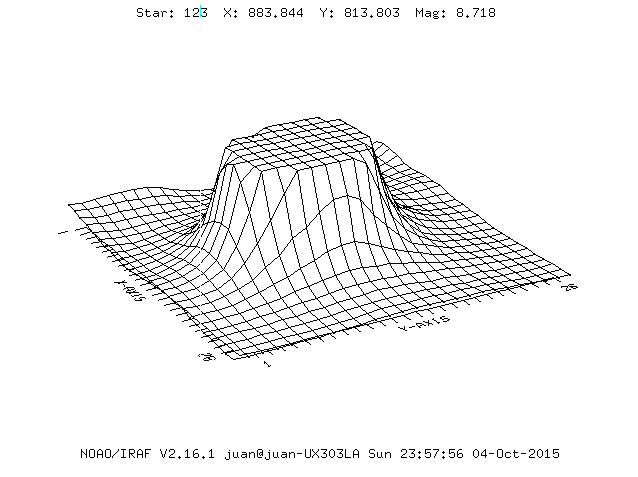
\includegraphics[width=12cm]{images/psf.png}
\caption[PSF modelling]{Some examples of the PSF modelling. The interactive mode allows us to accept of decline the result by pressing ``a" or ``d". In the top left and bottom right panels, the PSF can't be modelled correctly because they contain the contributions of various stars, the bottom left image is too saturated and is declined as well. The one at the top right has little noise and is the closest to a soft Gaussian behaviour (even though it is still a little saturated) so it can be accepted to model the PSF.}
\end{figure}

After running \textit{psf}, there will be created an image that contains the residuals of the psf modelling which can be seen in figure 3.10.

\begin{figure}[H]
\centering
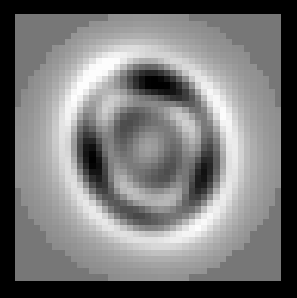
\includegraphics[width=5cm]{images/psf2.png}
\caption[PSF residuals]{PSF residuals}
\end{figure}

With the task \textit{seepsf} another image will be created but this time it will actually look like a star as shown in figure 3.11

\begin{figure}[H]
\centering
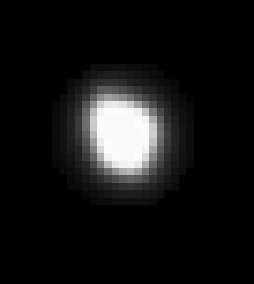
\includegraphics[width=5cm]{images/psf3.png}
\caption[PSF image created by the task Seepsf]{Seepsf converts a sampled PSF lookup table to a PSF image which can be visualized}
\end{figure}

Finally, after the modelling of the PSF was made, the task \textit{allstar} does the photometry of the cluster using the results we just stored in the current directory. The results of the PSF photometry gave us magnitudes smaller for those stars than the results given by the aperture photometry but there is a constant difference for all the stars which we can assume to be a calibration constant between the two methods. 

\begin{figure}[H]
\centering
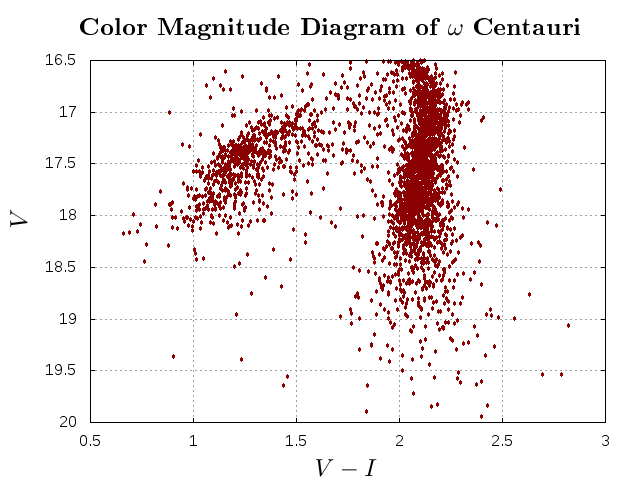
\includegraphics[width=12cm]{images/HR-diagram.png}
\caption[Pf]{Sd}
\end{figure}


\section{Spectroscopy}

This was the most important part of our observational data since it had the best quality we could obtain in the many domes of the observatory. Also, spectra of this kind is not easy to find in the scientific databases so we have important data to work with. The first spectroscopic procedures were also made for $ \omega $ Centauri cluster since we need to master the reduction and extraction techniques first in order to be able to start the scientific work about the mass modelling of the clusters.

\subsection{Spectroscopic Reduction}

The spectroscopic reduction is made by following some steps taking into account that we did not take any Skyflats so we need to create a response function using our dome flats. The steps are:

- First we make a Superbias combining all the bias frames and then we subtract it from all the lamp, targets and flat field frames.

- It was important to analyse the flats to see which ones are saturated, we consider that values over 65,000 counts (using implot) show saturated data. The ones that we could trust for May 14th were ten images called flats\_0012 to flats\_0021.

- The pre-superflat is made using the median given the number of images.

- We need to make a trimming in all images because there are some regions in the images that show unexpected luminosity, this is probably due to border errors in the camera or the obturator time of relaxation. The zones we decided to cut (in pixels) were [0-100] and [575-691].  

- A critical step is the creation of a response function, this is made by collapsing the pre-superflat to one column using \textit{blkavg}. The useful image for the creation of the Superflat is done by combining this column with \textit{blkrep}. This gives us an image that's uniformly distributed in the dispersion axis with the following IRAF commands.

blkavg MasterFlat.fits[1:475,*] AvgFlatCols 475 1

blkrep AvgFlatCols AvgFlatColsMaster 475 1

- The pre-superflat is now divided by the response function we created (AvgFlatColsMaster) and this gives us the Superflat that we will use to reduce our data.

- Finally, the task we use to remove the cosmic rays is \textit{lacos}, and it gives very accurate results, as it shows the ``mask" image with the removed cosmic rays.

Figures 3.13 and 3.14 show......The vertical axis of the spectra is the dispersion axis and the horizontal axis is the spatial separation between stars. To visualize the reductions we have the following figures taken from the dirty and reduced NGC5139 spectrum (Day of observation May 14th):

\begin{figure}[H]
  \centering
  \begin{minipage}[b]{0.45\textwidth}
    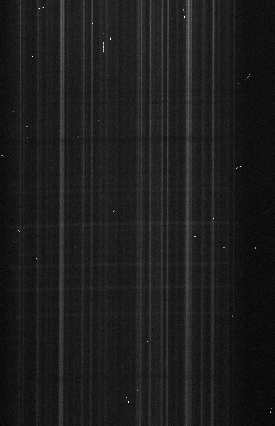
\includegraphics[width=\textwidth]{images/cluster_dirty.png}
    \caption[Dirty spectrum of NGC5139]{The dirty cluster spectrum has a small signal to noise ratio, besides border effects (such as a big gradient) that need to be trimmed and cosmic rays.}
  \end{minipage}
  \hfill
  \begin{minipage}[b]{0.45\textwidth}
    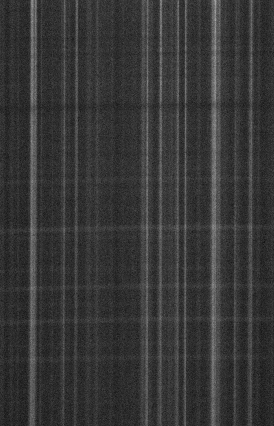
\includegraphics[width=\textwidth]{images/cluster_clean.png}
    \caption[Clean spectrum of NGC5139]{The clean spectrum without the bad data at the borders that needed to be trimmed, with a higher signal to noise ratio and the cosmic rays removed}
  \end{minipage}
\end{figure}

The images above are just a fraction of the whole image which is actually longer in the vertical direction, we show only a fraction for visual purposes. As we did not take skyflats, some telluric lines are visible even in the reduced spectrum but this can be solved doing a correct calibration and carefully examining the extraction of the spectra of the stars.

\subsection{Extraction}

Once the reduction is ready, we can proceed with the extraction of the spectra of the calibration stars and also the spectra of the stars in the clusters, this procedure is made with the task \textit{apall}. First, I did the extraction of the two calibration stars for each night of observation. For May 14th our calibration stars were HR4963 and HR4468 and for May 15th our calibration stars were HR4468 and HR7950.

Taking special care of correctly choosing the background, and with the following parameter configuration:

b\_number: 100
background: fit
weight: variance
saturate: 65215
rdnoise: 6
gain: 1

Interactively, one must choose very precisely the background regions to extract the spectrum and do the fitting routines with different orders until the best results are reached, the areas of the background are changed using the commands ``b" (for setting the background mode) and ``s" (for setting the range). A good choice for the background in the case of the calibration star is relatively easy but in the case of the extraction of the stars in the clusters one must take into account the high noise introduced by the other stars and the background so for every star one must zoom into the window using ``w" and ``a" between the boundaries of the range to be zoomed.

If a good choice of the background and the dispersion axis is well fitted, the task runs straightforward to get the spectrum of the star. In the case of the calibration lamps, the procedure is quite similar because the extraction of their spectrum is done with \textit{apsum}, which is very similar to \textit{apall}. 

For the calibration star HR4468, the extracted spectrum looks like the one shown in figure 3.15.

\begin{figure}[H]
\centering
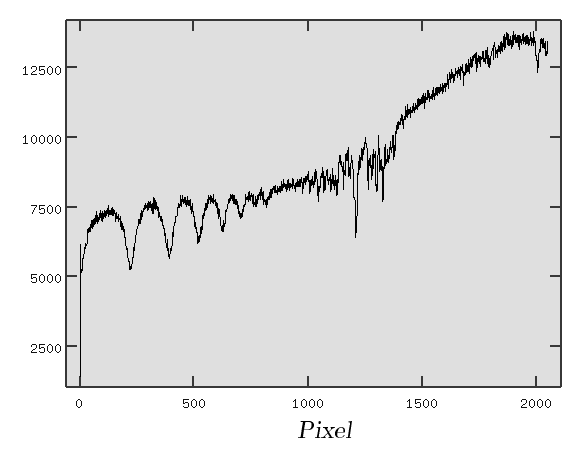
\includegraphics[width=9cm]{images/calib_star_apall.png}
\caption[Spectrum of calibration star HR4468]{Extracted spectrum of HR4468, note that the dispersion axis is still in terms of pixels instead of Angstroms, this is fixed by doing the wavelength calibration, also the direction will be shifted because the strong sodium absorption lines are in the left end of the spectrum and they should be in the right end}
\end{figure}

\subsection{Wavelength Calibration}

Once the spectrum is extracted, the following step is to calibrate it in wavelength in order to make it useful for scientific analysis. The wavelength calibration is made with the use of many tasks of IRAF like \textit{Identify}, \textit{Refspec} and \textit{Dispcor}. First, with \textit{identify} I use the interactive window in IRAF to select some prominent lines in the spectrum of the calibration lamps and assign them their correct wavelength using the theoretic spectrum of the lamp. In this case our calibration lamps were Ne-Ar (for May 14$^{th}$) and He-Ar (for May 15$^{th}$)  and OPD observatory provided us the theoretic distribution of emission lines of them. The lines look like the ones shown in figures 3.16 and 3.17

\begin{figure}[H]
  \centering
  \begin{minipage}[b]{0.45\textwidth}
    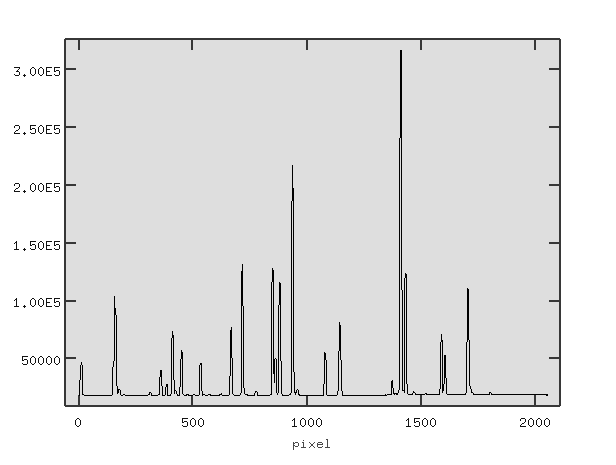
\includegraphics[width=\textwidth]{images/lamp_day1_2.png}
    \caption[Emission lines for the Ne-Ar calibration lamp]{Emission lines of the Ne-Ar calibration lamp that need to be wavelength calibrated ,the horizontal axis is in pixels and needs to be calibrated to units of wavelength}
  \end{minipage}
  \hfill
  \begin{minipage}[b]{0.45\textwidth}
    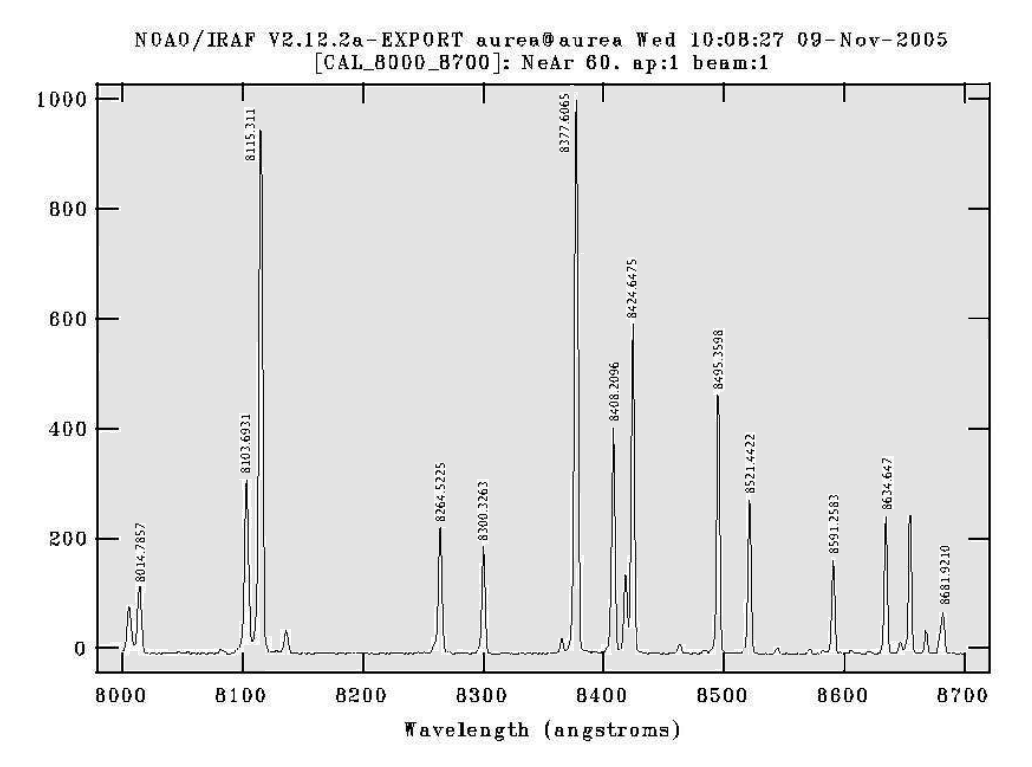
\includegraphics[width=\textwidth]{images/lamp1.png}
    \caption[Theoric emisison lines of a Ne-Ar lamp]{The theoretic emission lines of the Ne-Ar lamp provided by OPD that we use to make the wavelength calibration, note that the lines to be matched are going in the opposite direction}
  \end{minipage}
\end{figure}

Running \textit{identify} in the interactive mode and using ``m" to select the larger lines and typing the wavelength, the task creates a file stored in a new folder ``database" with the pixels with their corresponding values in units of Angstroms. After that, the targets (Calibration Stars and Globular Clusters) need to be calibrated with these files so it is necessary to edit their header to assign them the reference frames. It is enough to change the REFSPEC1 image key header on each lamp file in order to set the wavelength calibration. 

The task that actually does the calibration on wavelength for the science targets is \textit{dispcor}, it is only necessary to run the task over all the targets with their own wavelength calibrated lamp to get the calibrated spectrum which is the useful and important file to make the analysis of the width of the lines and their redshift.

The wavelength calibrated spectrum of the star HR4468, after running \textit{dispcor} is show in figure 3.18.

\begin{figure}[H]
\centering
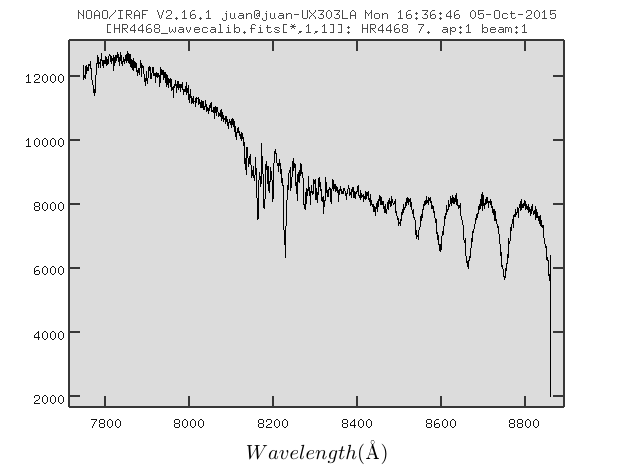
\includegraphics[width=8cm]{images/calib_star_wave.png}
\caption[Wavelength calibrated spectrum of HR4468]{The spectrum has been wavelength calibrated as we can see in the horizontal axis which is in units of Angstroms. Note that the strong absorption lines are now in the right part of the spectrum, this is because in the process of making the wavelength calibration, the direction of the axis was changed.}
\end{figure}

In order to see if the wavelength calibration (using the lamps spectra) was correct we used another technique consisting of using a sky spectrum (with no stars or contaminating objects) and identifying some of the atmospheric lines on it, the calibration of the science data is then made with the identified lines in this spectrum. This should be an accurate procedure since the spectrum of the sky is taken exactly with the same instrument and configuration than the science objects and it contains the same atmospheric lines that the GCs spectra. 

A secure way to extract the spectrum of the sky was using the original spectrum of a calibration star (reduced $HR4468$ in this case) and putting the aperture in an empty region in the image that does not contain any stellar absorption or emission lines. Of course the lines in the extracted spectrum are hard to identify so that the best way to do so is by looking at the already wavelength calibrated spectra of the star (calibrated with the comparison lamps) and identifying its prominent lines, then those lines had to be searched in the web to see how prominent they could be in the atmosphere and what their corresponding wavelength is. Once the information about the prominent emission lines is ready, one can identify them with the task \textit{identify} doing a careful zoom with ``w" and ``e"  in the sky spectrum. 

The same procedure consisting on saving a database file with the emission lines and changing the header of the image to calibrate needs to be done in order to complete the calibration.

We used this procedure to calibrate in wavelength $HR4468$ and see if both methods gave different results. The relevance of this procedure is that it allows us to see if we have any systematic problems or errors in the calibrations that would then affect our science data.

After the wavelength calibration was made for the stellar spectrum, we note a difference of around $0.65 \textrm{\AA}$ as we can see in figures 3.19 and 3.20.

\begin{figure}[H]
  \centering
  \begin{minipage}[b]{0.49\textwidth}
    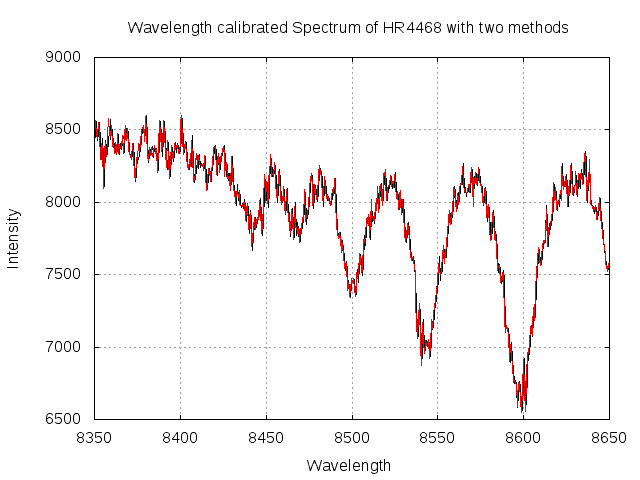
\includegraphics[width=\textwidth]{images/Espectros.png}
    \caption[Comparison between the two wavelength calibration methods]{Comparison between the two wavelength calibration methods. The black line is the spectrum of HR4468 calibrated with the lamp spectra and the red line is the same spectrum calibrated with the sky spectrum}
  \end{minipage}
  \hfill
  \begin{minipage}[b]{0.49\textwidth}
    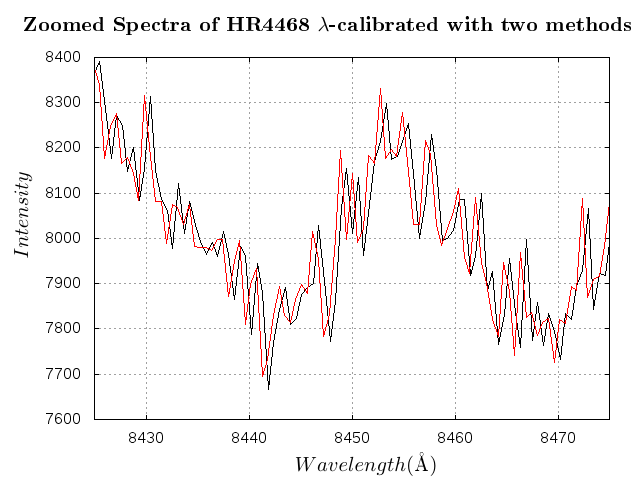
\includegraphics[width=\textwidth]{images/Espectros2.png}
    \caption[Zoomed comparison between the two wavelength calibration methods]{The same comparison zoomed in a small region to see the shift of the red and black lines. The difference is about 0.65$\textrm{\AA}$ in this region which could mean a difference of about $20km/s$ in the measured velocities for both spectra.}
  \end{minipage}
\end{figure}

What this shows is that the radial velocities that we compute may have a small systematic depending on the method we use for the wavelength calibration since even a small shift on the lines would be equal to a difference in velocities of tenths of kilometres per second, thus introducing a big systematic error in our data that would completely affect our modelling. The error bar in the velocities associated with the position of the lines of the spectrum is then too big to give us reliable information about the velocity dispersion in the inner region of the clusters so the calibrations have to be perfected.


\subsection{Flux Calibration}

This final part of the extraction and calibrations has the aim of calibrating the CCD chip response, spectrograph+telescope throughput and allow for atmospheric extinction. The result is a spectrum as observed from outside the atmosphere with an ideal uniformly sensitive detector+telescope+spectrograph. Basically, what the flux calibration does is, it takes from a tabular compilation the energy distribution of the standard star, it corrects this energy distribution for wavelength-dependent atmospheric extinction, it compares it to the energy distribution of the observed spectrum and derives from such a comparison the function that gives the response of our system for every wavelength.

The flux calibration takes place in three parts: Calibrating from the standard star, calculating the sensitivity function of the instrument, and finally, applying the calibration to the spectra. We will use the task \textit{observatory} to determine observatory parameters, \textit{standard} to flux calibrate each standard star, and \textit{sensfunc} to finally determine the wavelength response and the solution will be applied to the spectra by the task \textit{calibrate}.

In the first part, the calibration is made with one of the stars that are already included in IRAF, there are many stars so there's quite a good amount of options to choose. So the first task is the task \textit{standard}. The observatory parameter is specified as LNA (Laborat\'orio Nacional de Astrof\'isica) which is in IRAF's database. 

\textbf{The task standard}

The task standard determines calibration pass-bands and writes them to a file called ``std". The trick here is to specify the location of the the input extinction and flux calibration files. To do that, I edit the parameters of standard with the following routes:

Extinction file:                              onedstds\$/ctioextindt.dat

Directory containing calibration data:   onedstds\$ctionewcal/

Starname in calibration list:                l9239

Where I chose the Star l9239 because it has the spectral range that we use in our calibration Stars. And running the task interactively would be enough for this step.

\textbf{The task sensfunc}

The task \textit{standard} just recorded response of each standard star so the next step is to put the results together and find a proper wavelength dependence of instrumental sensitivity and atmosphere transparency using the task \textit{sensfunc}. It creates an image with a default name sens.0001. IRAF needs to have some general idea of atmospheric extinction before to start, so I set again extinct onedstds\$ /ctioextinct.dat.

Now, running the task interactively and taking into account that the function used to fit the instrumental response will be usually of very high order. A good idea is to use spline3 fitting (:function spline3) with some 20 pieces, i.e. (:order 20).
Finally ``q" exists the \textit{sensfunc} task and writes the sens.0001 image.

\textbf{The task calibrate}

The solution to each star to be calibrated is done with the task \textit{calibrate}. Editing the parameters of calibrate to set the appropriate extinction table: extinct onedstds\$ /ctioextinct.dat would be enough for this purpose. The task is run over all the wavelength calibrated spectra which had their airmass and other parameters appropriately set by the eso.set procedure. And finally it gives the flux-calibrated spectra ready for the relevant analysis concerning radial velocities.

After the flux calibration, I notice that the extremes of the spectra have irregularities given by the flux calibration procedures, but that can be cut because they don't have any relevant information. For the star calibration I create a new copy from pixel 45 to 1860, and the same y-range than the original image using imcopy:

\begin{center}
imcopy flux\_calib\_star\_fits[45:1860,*] cut\_flux\_calib\_star.fits
\end{center}

The wavelength and flux calibrated spectrum of the star HR4468, now ready to be used for radial velocities determination is displayed in figure 3.21.

\begin{figure}[H]
\centering
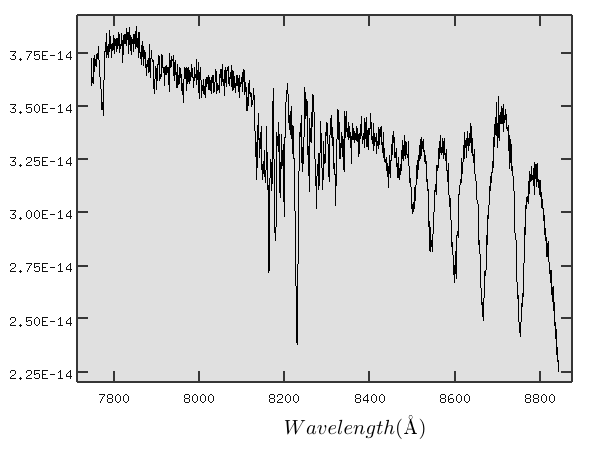
\includegraphics[width=8cm]{images/calib_star_flux.png}
\caption[Flux calibrated spectrum of HR4468]{Flux calibrated spectrum of HR4468 calibration star}
\end{figure}

In order to normalize the spectrum, first I find the maximum value in the spectrum using minmax and then I divide the whole image by this value. 

Something that can be very useful is to have the data of the spectrum in a different format so that it's information can be well used and analysed with simple programs like gnuplot, for this purpose, it is useful to create an Ascii table from the spectrum. For this purpose I need to first convert my image to a 1D image using the task \textit{scopy} and setting format=onedspec (this is only necessary if the spectrum was extracted in 2-D).

Now, with the image ready in 1-D, I use the task \textit{wspectext} to create the Ascii table like this:

\begin{center}
wspectext ready\_flux\_star.0001.fits normal\_cut\_flux\_star\_calib.txt
\end{center}

In principle, the same procedures hold for the star in the Globular Clusters, even though it must be made more carefully because the background noise and the crowded space surrounding them affects the spectra and it might change the values of the radial velocities, an example of a wavelength and flux calibrated spectrum of one of the stars in the NGC5139 cluster is shown in figure 3.22.

\begin{figure}[H]
\centering
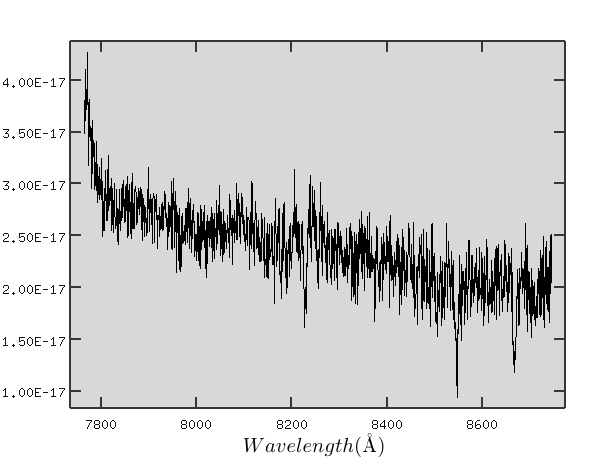
\includegraphics[width=8cm]{images/cluster_star_flux.png}
\caption[Spectrum of a prominent star of the NGC5139 globular cluster]{Spectrum of one of the most prominent stars in the NGC5139 cluster, after all the calibrations have been made}
\end{figure}

Although the noise is evidently higher than in the case of the spectrum of the calibration star, it is possible to see (even with the naked eye) two of the calcium strong absorption lines around 8543\AA$ $ and 8663\AA. After all of these procedures have been made to the important stars in the clusters and the calibration stars, the next step is to explore the best way to determine radial velocities with the use of some sophisticated tasks in IRAF such as \textit{RVSAO}, as we discuss in the next section. 

\section{Radial velocity determination}

In order to study the dynamics of the starts within the stellar systems we used various techniques with the spectroscopic data. One consists of extracting the spectrum of each individual star and measuring the shifting of the lines (with respect to the rest frame) to measure its radial velocity so that we can obtain the projected velocity dispersion; another technique consists of using the full integrated spectrum of each cluster and measure the Doppler broadening of the lines (as shown in Figure 2.9) to directly get information about the velocity dispersion with respect to a rest frame template. 

Our radial velocity determination started with the first technique (analysing spectra of individual stars) with the IRAF package RVSAO:

\subsection{RVSAO}

This package is the radial velocity analysis package of the Smithsonian Astrophysical Observatory and is intended to properly organize a set of programs to obtain redshifts and radial velocities from spectra. It contains (by 2015) 26 programs well documented for the users' need. We focus on the task XCSAO as well as the utilities of EMSAO and BCVCOR for our set of data.

The program XCSAO is the most important one in the RVSAO package, it implements the cross-correlation method and interactive algorithms to properly prepare the spectra for a correct radial velocity analysis such as the removal of the continuum and the emission line suppression. For using this task, one must provide the spectrum of the object and a template spectrum (preferably in the rest frame so that the emission and absorption lines are in their proper wavelength) that will be used for the cross correlation, it also requires the starting and ending wavelength, the type of Fourier filtering and many other details according to the user's desires and interests.

By using one of IRAF's templates \textit{``habtemp0.fits"} that covers the range of 2884.1547$\textrm{\AA}$ to 7037.3375$\textrm{\AA}$ we can directly run XCSAO on a stellar spectrum that will use the Fourier transform to cross correlate them and give an approximate value of the radial velocity of the star an printed in an irafterm window as seen in figure 3.23. 

\begin{figure}[H]
\centering
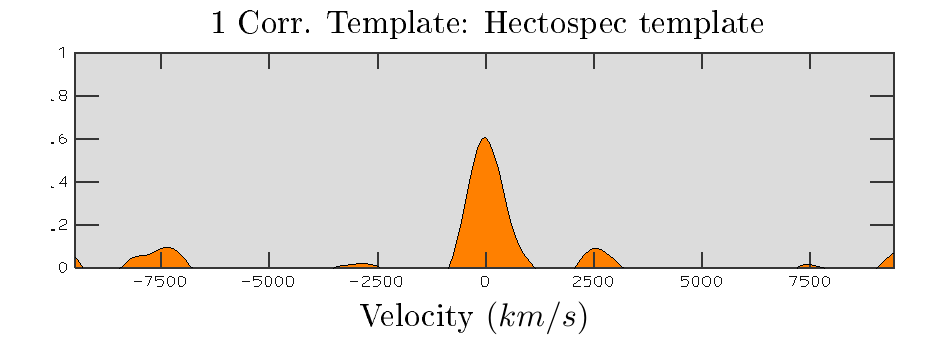
\includegraphics[width=10cm]{images/xcsao.png}
\caption[XCSAO results]{The relevant part of XCSAO results, the cross correlation in this case is god and shows a well-behaved peack, the radial velocity of the star in this case is around $-30km/s$}
\end{figure}

The results of RVSAO have a really strong dependence on the quality of the template used for the cross correlation, and some of the IRAF spectra have different wavelength ranges and flux values on the characteristic lines so that they won't give reliable results. One is forced to create a template spectrum with the most prominent lines to be used to correlate the object spectrum. One task that can be very useful in the creation of the templates is \textit{rspectext} that creates an image spectrum from an ascii table where the user can set the dispersion to be assigned to the spectra, and the appropriate values for the flux and intensity of absorption or emission lines.

One of our created templates that holds information about some absorption lines including the calcium triplet and made using \textit{rspectext} is shown in the following figure:

\begin{figure}[H]
  \centering
  \begin{minipage}[b]{0.5\textwidth}
\begin{table}[H]
\begin{center}
  \begin{tabular}{| c|  c|  c| }
    \hline
    Wavelength & Intensity & Line \\ \hline
    8497.84 & -0.8 & CaII \\
    8542.09 & -0.89 & CaII \\
    8598.49 & -0.872 & HI \\
    8661.74 & -1.0 & CaII \\
    8750.91 & -0.97 & HI \\
    \hline
  \end{tabular} 
    \end{center}
\caption[Imput data for the creation of template with rspectext]{Imput data for the creation of template with rspectext, the values of the intensity of the absorption lines are determined by the user according to the strength or the features involving the stellar spectra, the name of the lines is not relevant for the creation of the template}
\end{table}
  \hfill
    \end{minipage}
  \begin{minipage}[b]{0.49\textwidth}
    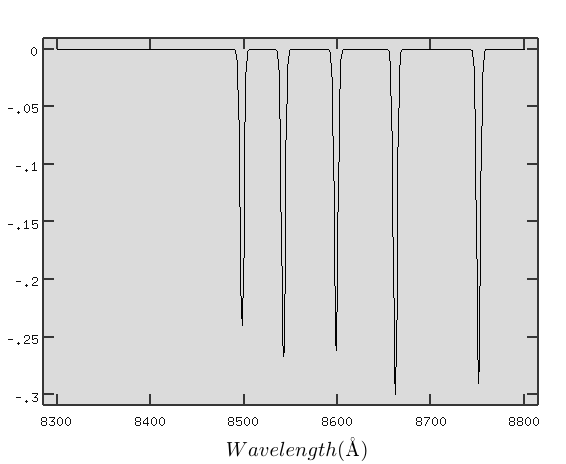
\includegraphics[width=\textwidth]{images/template.png}
    \caption[Results of the template spectrum created by rspectext]{Results of the template spectrum created by rspectext in the given wavelength range, this template does not have any emission lines since our spectra didn't have strong emission features.}
  \end{minipage}
\end{figure}

Another important issue to be addressed when we analyse radial velocities is the fact that our ground based observations are done in a moving system around the Sun and around the galaxy so that the Doppler shift of the lines would be affected by this relative movement of the Earth with respect to the Sun's velocity that the Earth is attached to. The issue can be seen in the following figure.

\begin{figure}[H]
\centering
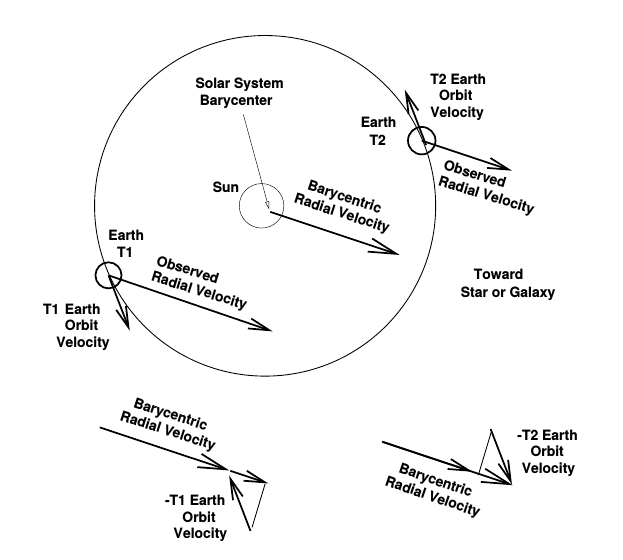
\includegraphics[width=10cm]{images/bcvcor.png}
\caption[The nature of the barycenter shift of radial velocities]{Correction of radial velocity observed from the earth to the radial velocity observed from the center of mass of the solar system shown at two different times in the earth's orbit, M. Kurtz, D. Mink 1993 \cite{1}}
\end{figure}

The barycenter correction of the spectra can be made using the task BCVCOR, the task calculates the correction of the barycenter velocity according to the date of the observation and edits the header of the image so that this information will be stored and read by other tasks like XCSAO by the time the radial velocity calculation is to be made. Another important task of the RVSAO package is EMSAO that computes redshifts by identifying shifted emission lines in the spectrum with respect to templates with emission lines in the rest frame. This task might be very useful if the spectra has strong emission features but the cross correlation techniques used by XCSAO might give a better choice if the spectrum has important absorption lines.
As seen in the following figure, EMSAO identifies the strong features of the spectrum to be measured using files in the IRAF database that contain information about emission lines with their given wavelength:   

\begin{figure}[H]
\centering
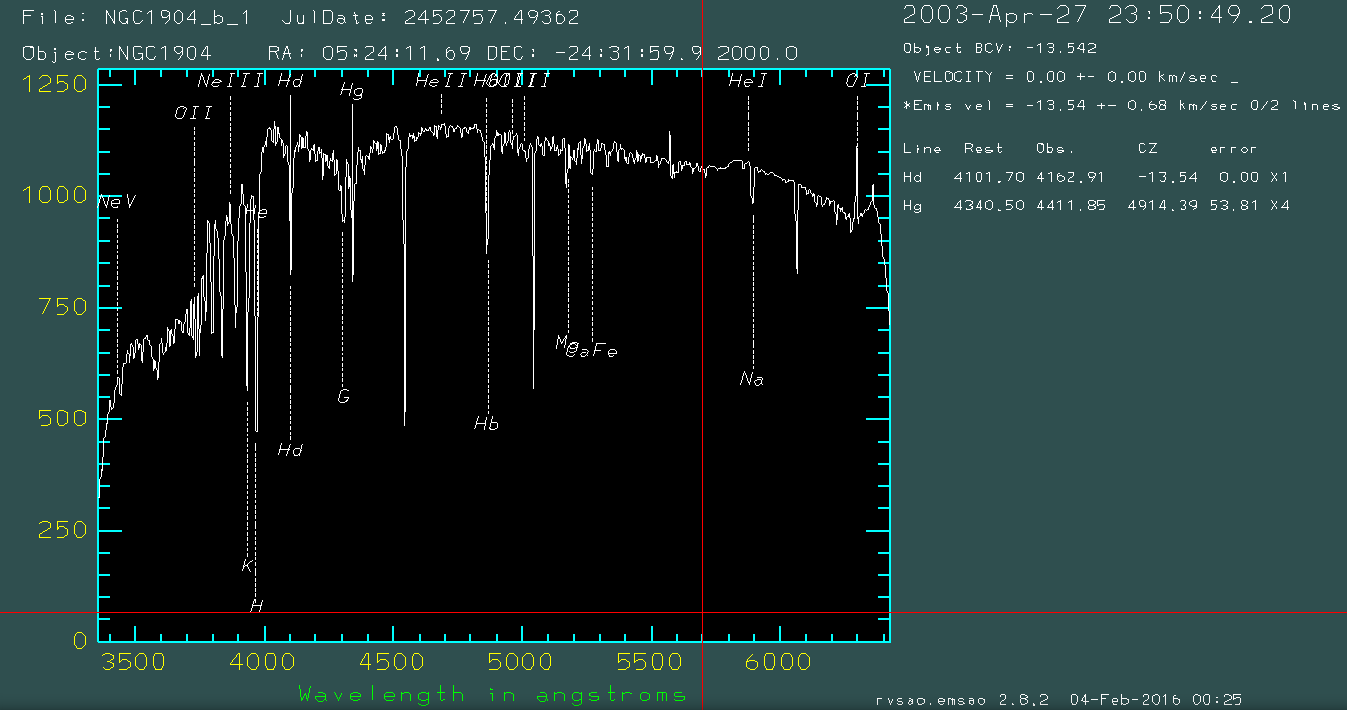
\includegraphics[width=13cm]{images/emsao.png}
\caption[EMSAO results with the identification of lines]{EMSAO results with the identification of strong absorption lines in the integrated spectrum of the Globular Cluster NGC1904 but few emission, note that the spectrum has already a barycentric velocity correction (BCV) of $-13km/s$, specified in the header as explained before.}
\end{figure}

One of the other techniques we used to study velocity dispersions in GCs spectra was using another IRAF task that also uses cross correlation techniques like XCSAO but runs much more straightforward and has a strong advantage regarding the output information after the fitting is made, the task is FXCOR. 

\subsection{FXCOR}

This IRAF package, very useful for radial determination decomposes every signal in a sum of sinusoidal functions through the Fourier transformation of a spectrum that has been wavelength calibrated. The product of the transformed signals generates the correlation function, which is similar to a Gaussian function and displayed in the irafterm after the task has been run. The stronger the correlation is, the higher the peak of the curve is, to a maximum of 1 (for the perfect correlation) in the case of an autocorrelation. Regarding the results of the correlation, the peak height is index of the superposing grade of the two spectra because it depends on the presence of the same absorption (or emission) lines as explained by V. Guglielmo et al. 2009 \cite{16}. 

\begin{figure}[H]
\centering
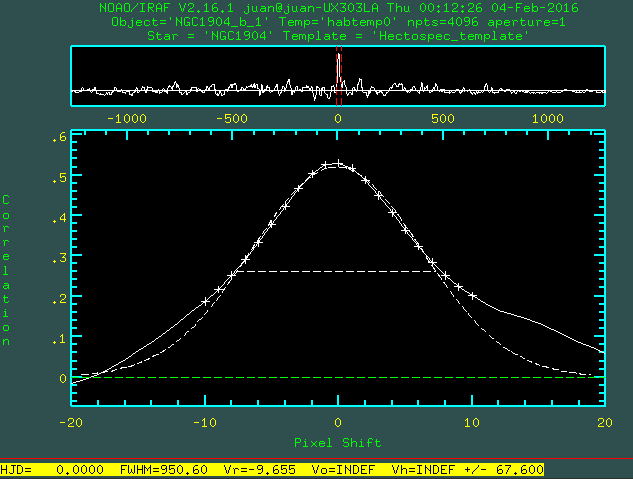
\includegraphics[width=10cm]{images/fxcor.png}
\caption[FXCOR results for NGC1904]{FXCOR cross correlation results for NGC1904 with the IRAF template habtemp0 with a measured radial velocity of $-9.655km/s$, note that the peak has a well-behaved shape and it is the strongest peak so that the correlation gave good results.}
\end{figure}

Besides the radial velocity calculation made by this task, for our purposes its most important feature is the fact that it also measures the width of the peak at the middle height (FWHM), which is useful to calculate the velocity dispersion of integrated spectra with the following relations:

The first thing we have to do is calculate the intrinsic FWHM$_{i}$, which is in terms of the FWHM of the correlation and the FWHM of the autocorrelation of the object spectrum (FWHM$_{a}$):

\begin{equation}
FWHM_{i}=\sqrt{{FWHM^{2}}-{FWHM_{a}^{2}}}
\end{equation}

With the intrinsic FWHM$_{i}$, the velocity dispersion give by the object spectrum is given by:

\begin{equation}
\sigma=\frac{FWHM_{i}}{2.35}
\end{equation}

And thus, using the virial theorem to relate the kinetic to the potential energy one can calculate the mass of the mass of the object (GCs in our case) is given by:

\begin{equation}
M=\frac{r_{e}\sigma^{2}}{0.33G}
\end{equation}

With $r_{e}$ the half mass radius (where half of the galaxy light is contained)

Our radial velocity determination involves the necessity of creating or finding very accurate templates because as it has been mentioned, the results of the correlation are highly dependent on the quality of the absorption and emission lines in them.   


\section{More data}



\begin{table}[H]
\begin{center}
\begin{tabular}{| c | c| }
    \hline
    \textbf{Article} & \textbf{Mass} ($M_{\odot}$) \\ \hline
    Mandushev et al. 1991 & $2.4 \times 10^{6}$  \\ \hline
    Pryor \& Meylan & $3.98 \times 10^{6}$  \\ \hline
    Meylan et al. 1995 & $5.1 \times 10^{6}$  \\ \hline
    Majewski et al. 2000 & $5.1 \times 10^{6}$  \\ \hline
    Van de Ven et al. 2006 & $2.5 \times 10^{6}$  \\ \hline
    Cassini et al. 2009 & $3.0 \times 10^{6}$  \\ \hline
    Valcarce \& Catelan, 2011 & $3.0 \times 10^{6}$  \\ \hline
    Jalali et al. 2011 & $2.5 \times 10^{6}$  \\
    \hline
  \end{tabular} 
\caption[Mass Omega Centauri]{Reported values of Omega Centauri's dynamical mass}
\end{center}
\end{table}